\chapter{Evaluation}

In the previous chapter, the implementation characteristics of an actor-based Web framework were observed from the view of a developer (see chapter \ref{sec:impl}). While these aspects are important during the development of an application, once the application is publicly accessible, performance is a paramount factor. This chapter documents tests conducted with respect to performance criteria defined in chapter \ref{lab:technical} -- for example request frequency and response time (see section \ref{lab:frequency}) -- and aims to define use-cases for synchronous and asynchronous application structure in the context of Web frameworks.

\section{Prerequisites}

Modern Web server performance can be defined by the system's behaviour when processing a high number of simultaneous requests. Ideally, the response time for each request should be as low as possible and should not increase significantly with the number of simultaneous requests. 

To test the behaviour of thread-based applications side by side to event-based applications, tests should preferably be conducted under very similar conditions, the only major difference being asynchronous processing. Since in section \label{lab:lang} the \textit{Play!} framework was identified  as a feasible choice for demonstrating asynchronous processing in Web frameworks, \textit{Play!} is also used in the following performance tests. To achieve comparable performance, the thread-based contender application should ideally also be run on the \textit{Java} virtual machine (JVM). This leaves numerous choices; however, the \textit{Spring MVC}\footnote{\url{http://spring.io/}} framework is considered a similar solution regarding application structure and runtime behaviour \cite[p. 109]{Scala}.

\section{Testing}

Methodology


Independent, but identical systems

Netty vs Jetty
Iterative Fib proved to be most suitable (tail recursion)
Java VM 7
Not too much load, equal reliability

\section{Results}

\begin{figure}
\centering\small
\setlength{\tabcolsep}{0mm}
  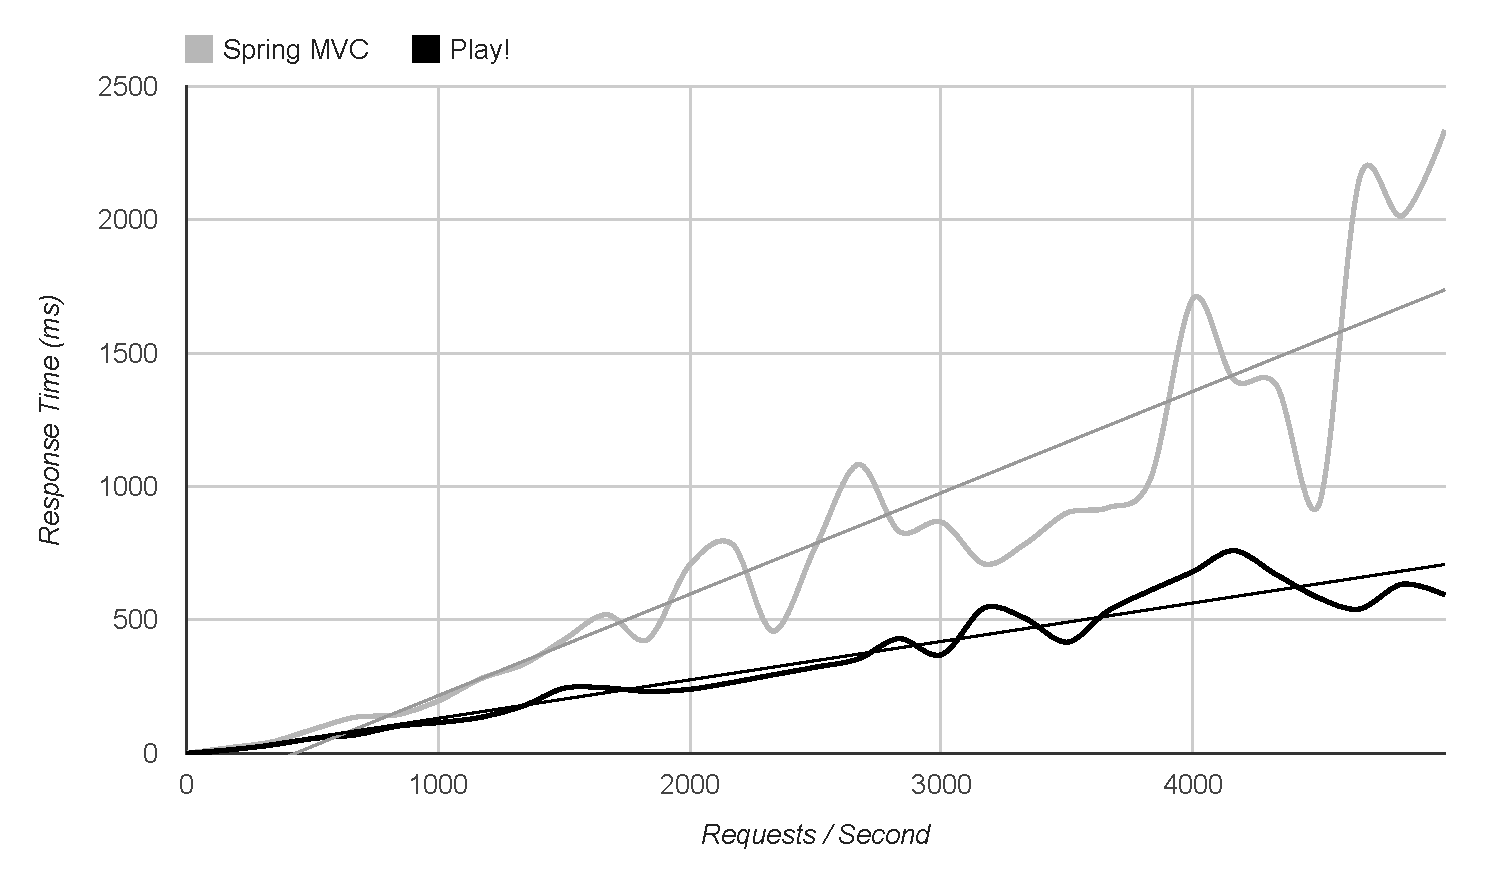
\includegraphics[width=.99\textwidth]{onsystem01test}
\caption{fib(1000)
}
\label{fig:response_time} 
\end{figure}

\begin{figure}
\centering\small
\setlength{\tabcolsep}{0mm}
  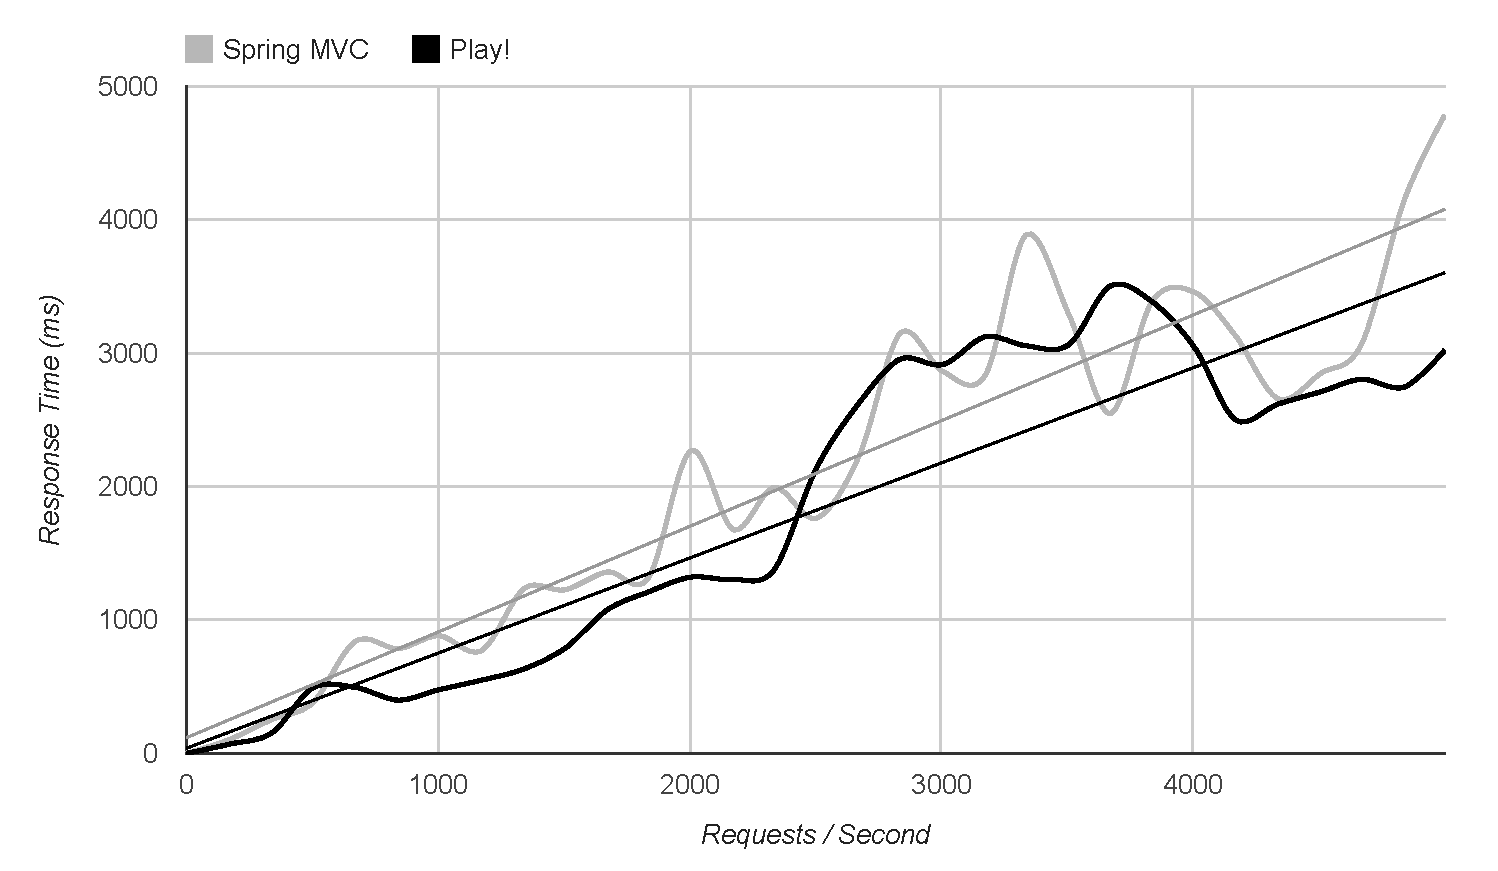
\includegraphics[width=.99\textwidth]{onsystem02test} 
\caption{fib(5000)
}
\label{fig:response_time} 
\end{figure}

\begin{figure}
\centering\small
\setlength{\tabcolsep}{0mm}
  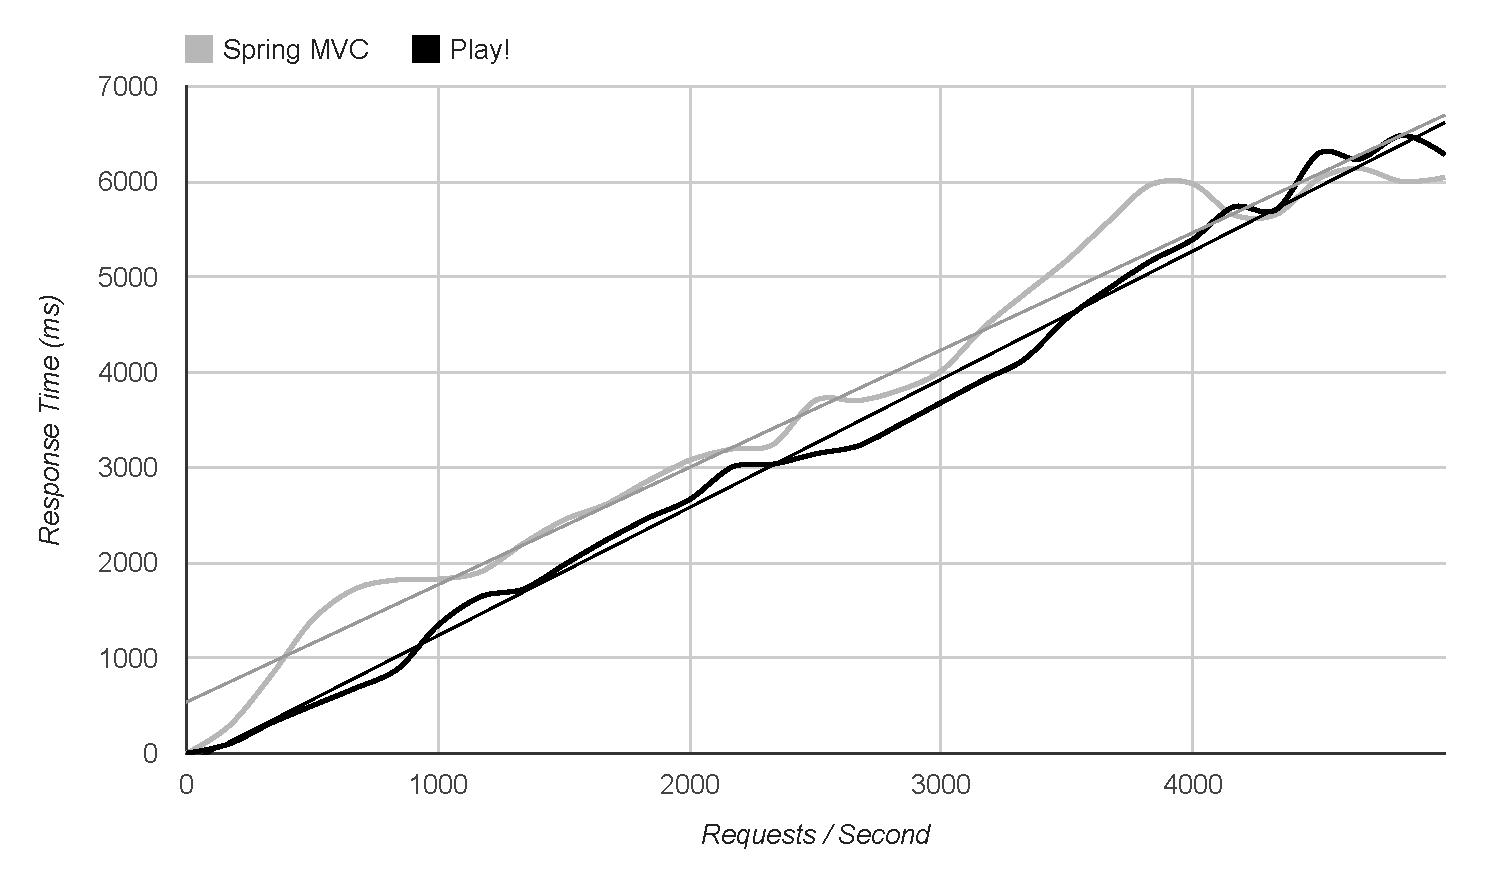
\includegraphics[width=.99\textwidth]{onsystem03test}
\caption{fib(10000)
}
\label{fig:response_time} 
\end{figure}

\begin{figure}
\centering\small
\setlength{\tabcolsep}{0mm}
  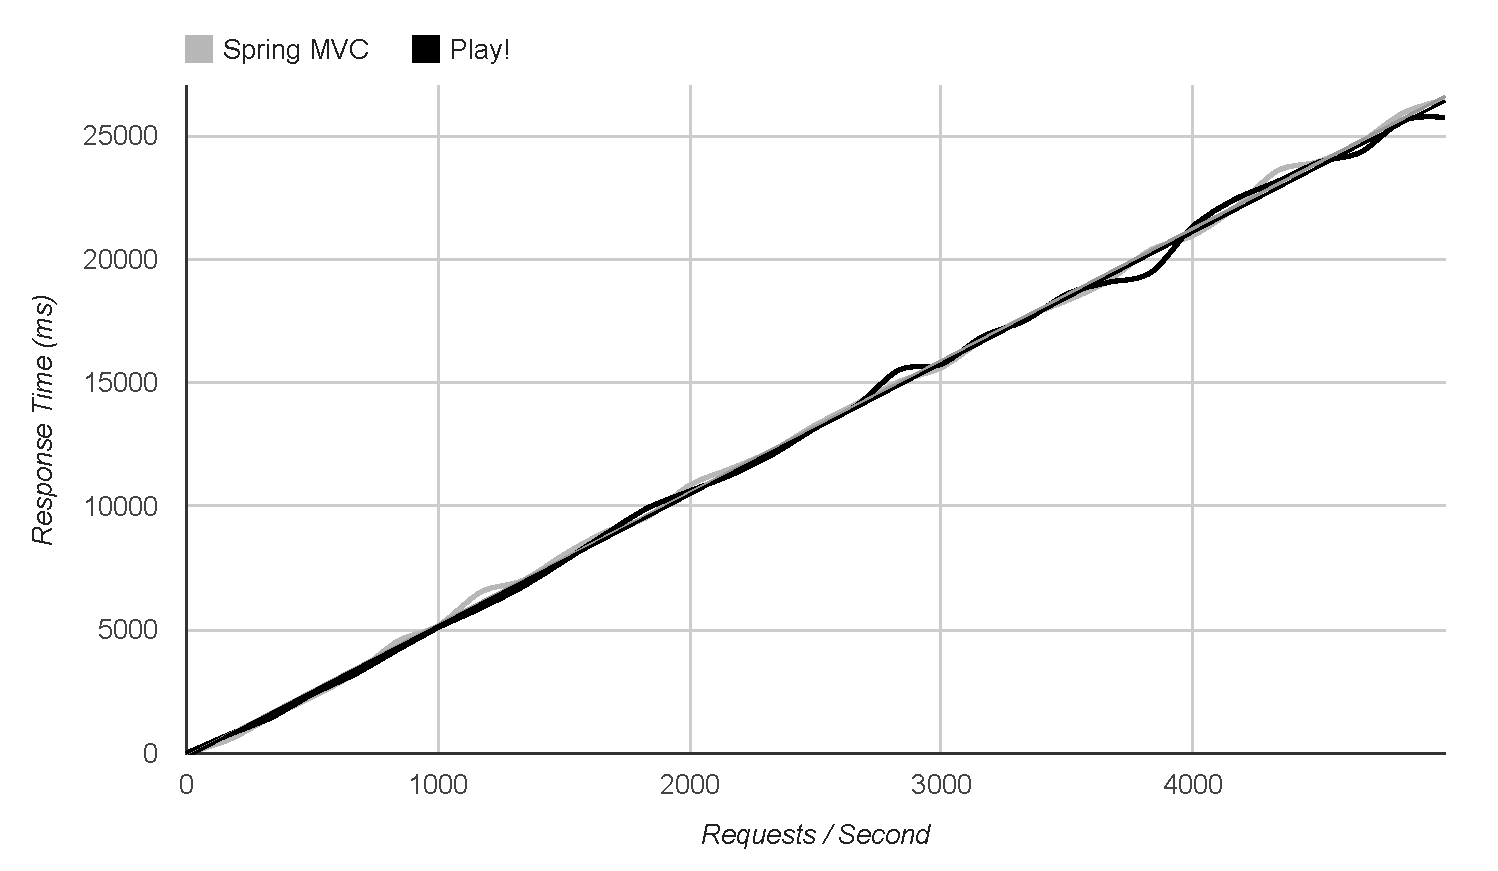
\includegraphics[width=.99\textwidth]{onsystem04test}
\caption{fib(50000)
}
\label{fig:response_time} 
\end{figure}

\begin{figure}
\centering\small
\setlength{\tabcolsep}{0mm}
  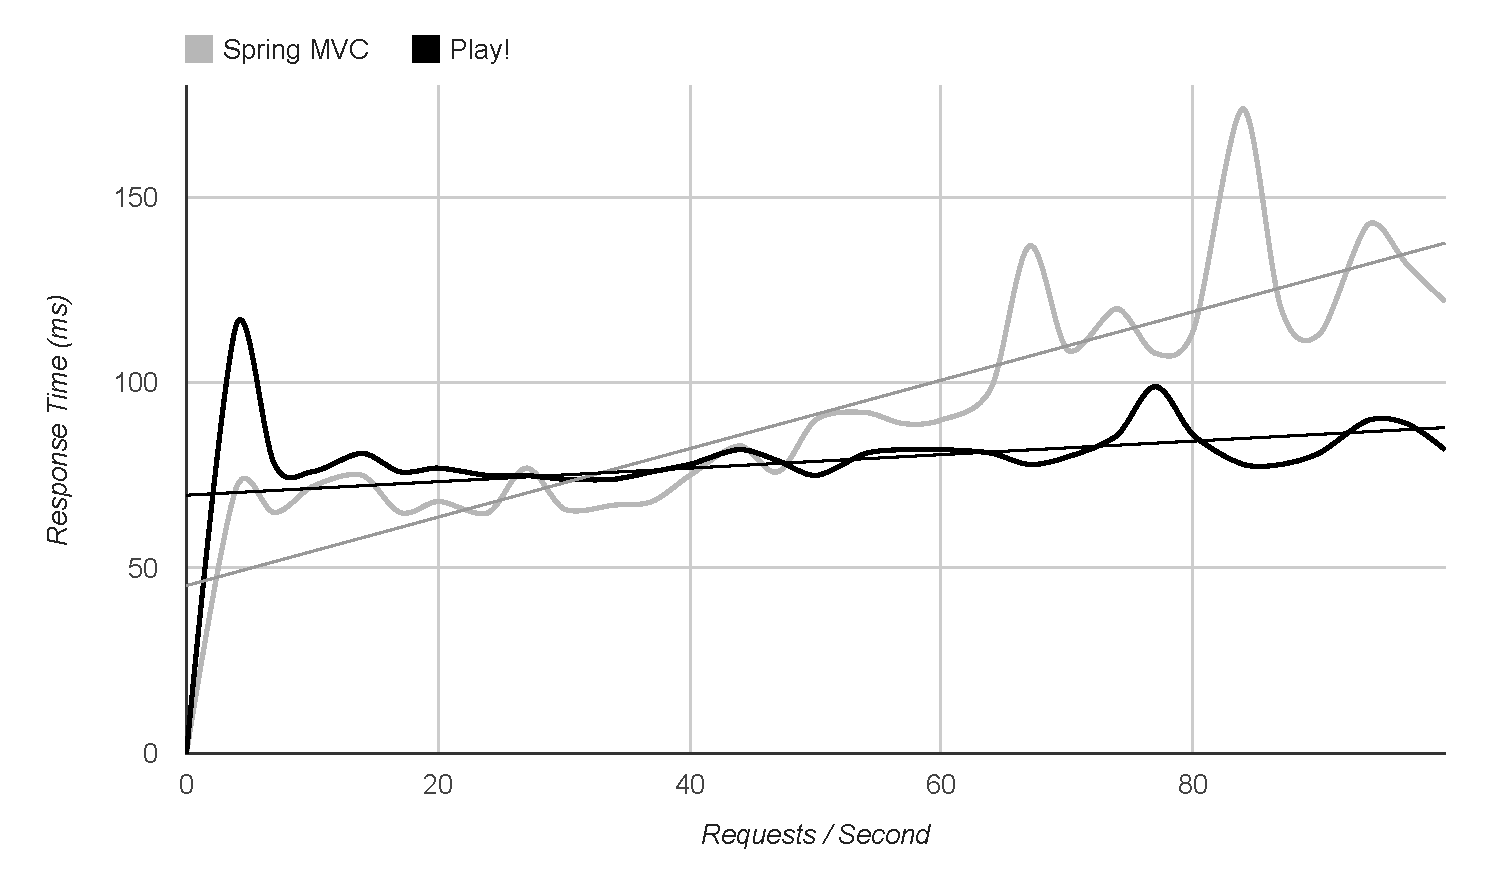
\includegraphics[width=.99\textwidth]{offsystem01test}
\caption{web(100)
}
\label{fig:response_time} 
\end{figure}

\begin{figure}
\centering\small
\setlength{\tabcolsep}{0mm}
  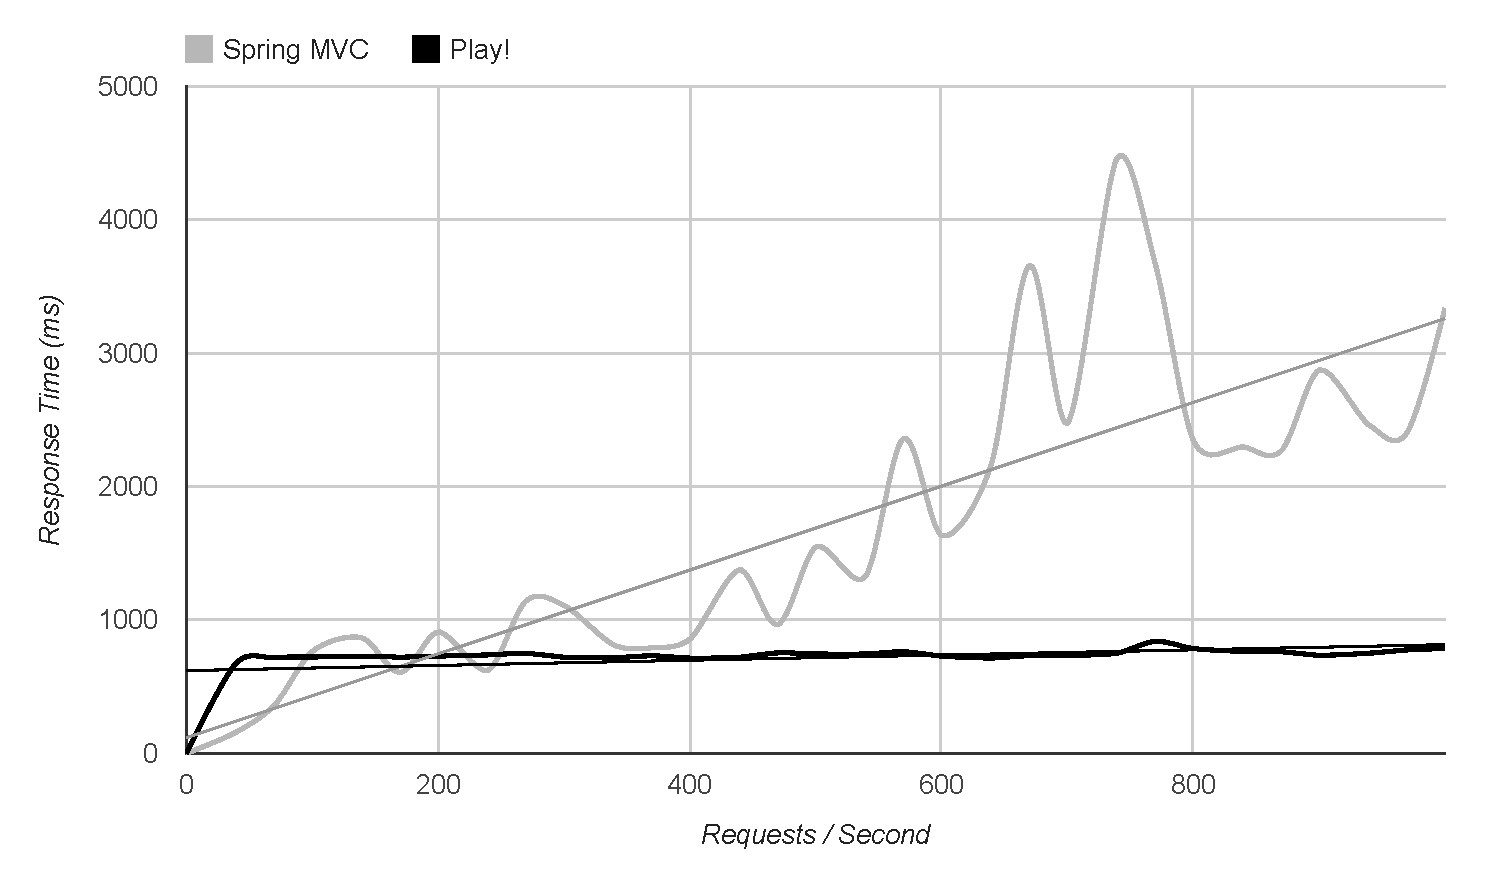
\includegraphics[width=.99\textwidth]{offsystem02test}
\caption{web(1000)
}
\label{fig:response_time} 
\end{figure}

\begin{figure}
\centering\small
\setlength{\tabcolsep}{0mm}
  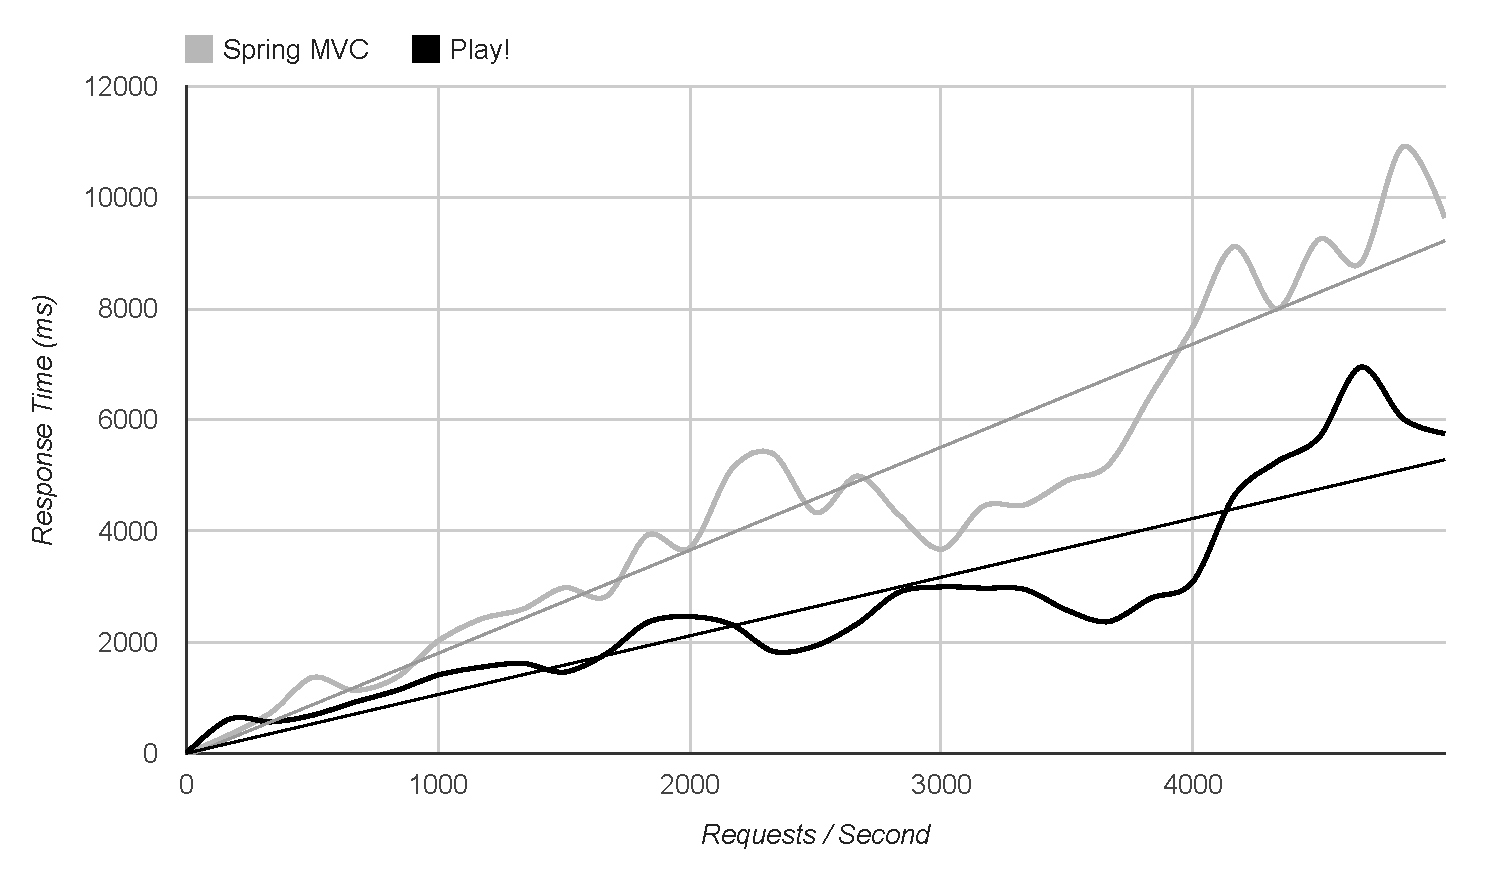
\includegraphics[width=.99\textwidth]{offsystem03test}
\caption{web(5000)
}
\label{fig:response_time} 
\end{figure}

JMeter
loader.io

\section{Interpretation}
On-system operations!!
=> at maximum load, equal outcome from a certain point on

Off-system operations? DB? Web?